\begin{center}
{\fontsize{11}{13}\selectfont \textbf{Общая характеристика работы}}
\end{center}

\newcommand{\actuality}{\underline{\textbf{\actualityTXT}}}
\newcommand{\progress}{\underline{\textbf{\progressTXT}}}
\newcommand{\aim}{\underline{{\textbf\aimTXT}}}
\newcommand{\tasks}{\underline{\textbf{\tasksTXT}}}
\newcommand{\novelty}{\underline{\textbf{\noveltyTXT}}}
\newcommand{\influence}{\underline{\textbf{\influenceTXT}}}
\newcommand{\methods}{\underline{\textbf{\methodsTXT}}}
\newcommand{\defpositions}{\underline{\textbf{\defpositionsTXT}}}
\newcommand{\reliability}{\underline{\textbf{\reliabilityTXT}}}
\newcommand{\probation}{\underline{\textbf{\probationTXT}}}
\newcommand{\contribution}{\underline{\textbf{\contributionTXT}}}
\newcommand{\publications}{\underline{\textbf{\publicationsTXT}}}

\textbf{Актуальность темы.}
На сегодняшний день взаимодействие человека с компьютерными системами через управление речевыми командами является одним из самых удобных и перспективных форматов.

% версия для автореферата
%Первая попытка конструирования системы автоматического распознавания речи была сделана в 1952 году, а уже в 1970-е годы исследования в области распознавания речи достигли значительных успехов.
%До настоящего времени распознавание речи совершенствовалось, а словарь распознаваемых слов вырос до нескольких десятков тысяч.
%Применение быстрых методов декодирования позволило производить распознавание в реальном времени.

% версия для диссертации
Первая попытка конструирования системы автоматического распознавания речи была сделана в 1952 году в Bell Laboratories, США~\cite{davis1952automatic}.
Система с хорошим уровнем точности распознавала цифры от нуля до девяти, произнесённые диктором через телефонный автомат.
Значительные улучшения качества в области распознавания речи были достигнуты в 70-ых годах.
В то время технологии автоматического распознавания отдельных команд основывалась на работах Itakura в США~\cite{itakura1975minimum}, Sakoe и Chiba в Японии~\cite{sakoe1978dynamic} и Величкина и Загоруйка в СССР~\cite{velichko1970automatic}.
Советские учёные производили улучшения методов распознавания с помощью эталона.
Применение подхода динамического программирования было отличительной особенностью японского исследования.
Работа Itakura раскрыла метод кодирования линейного предсказания (Linear Predictive Coding, LPC), который успешно использовался в распознавании сигналов с низким битрейтом (количество битов информации, передаваемых в секунду).
В AT\&T Bell Laboratories были построены распознающие системы, обработка акустического сигнала в которых была основана на LPC анализе, а процесс распознавания проходил с использованием метода динамической трансформации времени (Dynamic Time Warping, DTW).
В 1980-х годах от подходов, основанных на применении эталонов, научные работы в области распознавания речи перешли к моделированию статистическими методами.
Использовались скрытые модели Маркова (Hidden Markov Models, HMM).
Работы Бейкера~\cite{baker1990stochastic} были одними из первых, в которых для решения задачи распознавания речи были применены HMM.
С 1990-х годов распознавание речи несколько усовершенствовалось.
Словарь распознаваемых слов вырос до нескольких десятков тысяч.
Использование быстрых методов декодирования позволило производить распознавание в реальном времени.
В современных дикторозависимых системах, распознающих отдельные слова, количество которых достигает двадцати тысяч слов, ошибки составляют менее 0.1~\%~\cite{das1993influence}.
И около 5~\% ошибок в независимых от диктора системах, которые распознают слитную речь из тысячи слов~\cite{aubert1993continuous}.

В современных системах применяются 3 основные группы методов распознавания речи.
Первая группа --- это скрытые марковские модели.
В них входная речь рассматривается как последовательность фонем с определёнными вероятностями перехода.
Распознавание производится через поиск наиболее вероятной последовательности фонем для данного входного сигнала.
Вторая --- это методы, основанные на сравнении с эталоном.
Для каждого слова из словаря некоторым образом составляется эталон.
При распознавании выбирается то слово, эталон которого наиболее близок к входному сигналу.
Третья группа методов основана на искусственных нейронных сетях.
Суть методов состоит в нахождении такой решающей функции, которая по входному сигналу может определить его принадлежность к определённому классу.
Искусственные нейронные сети построены по принципу организации биологических нейронных сетей и хорошо справляются с широким спектром задач.

В данной работе решается задача повышения вероятности правильных распознаваний и снижения влияния акустических шумов путём разработки и совершенствования алгоритмов распознавания команд речевого интерфейса пилота для управления бортовым оборудованием современных самолётов.
По сравнению с обычной задачей распознания речи к речевому интерфейсу кабины пилота предъявляются следующие требования:

\begin{itemize}
	\item распознавание ограниченного словаря из слов или фраз;
	\item компактность, автономность, высокое быстродействие;
	\item хорошее качество распознавания в условиях сильного шума.
\end{itemize}

% версия для автореферата
%С учётом этих требований широко используемые скрытые марковские модели не подходят из-за низкого качества распознавания в условиях шума.
% версия для диссертации
С учётом этих требований широко используемые скрытые марковские модели не подходят из-за низкого качества распознавания в условиях шума \cite{korsun2013experimental}.

Остальные две группы методов в настоящий момент не обеспечивают необходимой надёжности распознавания.
По этой причине тема настоящей работы, направленной на совершенствование методов распознавания речевых команд с помощью сравнения с эталоном и с использованием нейронных сетей, является актуальной.
Исследования, выполненные в рамках данной работы, направлены на решение таких практически значимых и актуальных задач, как предобработка входящего сигнала путём выделения однородных частей, улучшение качества эталонов с помощью выделения в них главных компонент и использование систем распознавания из нескольких эталонов.
В работе также проведено обширное экспериментальное исследование всех разработанных методов на различных наборах входных данных с несколькими уровнями шума.

\textbf{Объект и предмет исследования.}
В работе в качестве объекта исследования рассматриваются речевые команды, а предметами исследования являются методы и алгоритмы распознавания речевых команд.

\textbf{Целью} работы является повышение вероятности правильных распознаваний и снижение влияния акустических шумов, путём разработки алгоритмического обеспечения для распознавания команд речевого интерфейса кабины пилота в виде отдельных слов и фраз.
За рамками работы остались выбор оптимального состава команд и их интерпретация.

Для достижения поставленной цели решаются следующие научно-технические задачи:
\begin{itemize}
	\item анализ статистических свойств речевых команд и их нормализация;
	\item разработка алгоритмов предварительного разбиения записей на однородные части;
	\item разработка алгоритмов исключения шума и выделения наиболее значимых компонент в эталоне;
	\item исследование статистических закономерностей верного и неверного распознавания речевых команд и их использование для уменьшения количества ошибок;
	\item разработка алгоритмов использования нескольких эталонов одного слова для улучшения качества распознавания;
	\item исследование современных типов и архитектур искусственных нейронных сетей глубокого обучения для применения в задаче распознавания речевых команд.
\end{itemize}

\textbf{Методология и методы исследования.}
Основными методами исследования, используемыми в работе, являются: анализ данных, цифровая обработка сигналов, теория вероятностей, математическая статистика, численная оптимизация, проектирование программных средств.

\textbf{Научная новизна} заключается в разработке совокупности алгоритмов, обеспечивающих повышение вероятности правильных распознаваний команд речевого интерфейса кабины пилота:
\begin{itemize}
	\item алгоритм разбиения речевых команд на фонетически однородные части на основе модифицированного метода динамического программирования;
	\item алгоритм оптимизации эталонов на основе метода главных компонент;
	\item алгоритм оптимизации размерности параметрических портретов с использованием полиномов Чебышёва;
	\item алгоритм распознавания команд по нескольким эталонам с использование байесовского подхода и метода комитетов;
	\item алгоритм распознавания команд нейронными сетями глубокого обучения, способных обучаться на выборках малого размера.
\end{itemize}

\textbf{Практическая значимость.}
Полученная в результате работы совокупность алгоритмов обеспечивает высокую точность распознавания речевых команд при различных уровнях шума, в том числе с учётом случая статически неустойчивого самолёта.
Результаты работы могут быть применены в учебном процессе и в ходе разработки алгоритмического обеспечения речевого интерфейса пилота для таких задач, как отображение информации, выбор частоты радиооборудования, прокладка маршрута, управление системой опознавания и датчиками, запрос запаса топлива.

\textbf{Положения, выносимые на защиту:}
\begin{enumerate}[label={\arabic*)}]
	\item Разработан алгоритм разбиения речевых команд на фонетически однородные части, отличающийся от существующих применением модифицированного метода динамического программирования.
	\item Разработан алгоритм оптимизации эталонов, отличающийся от существующих тем, что искомый эталон формируется как линейная комбинация главных компонент, оптимизирующая заданный критерий качества.
	\item Разработан алгоритм оптимизации размерности параметрических портретов, отличающийся выделением наиболее значимых составляющих с использованием полиномов Чебышёва.
	\item Разработан алгоритм распознавания команд по нескольким эталонам, отличающийся применением последовательного оценивания с расчётом апостериорных байесовских вероятностей.
	\item Разработан алгоритм распознавания команд нейронными сетями глубокого обучения, отличающийся от существующих обучением на выборке малого размера.
\end{enumerate}

\textbf{Достоверность результатов} обеспечивается корректным применением математической статистики, методов идентификации и анализа данных, подтверждением полученных теоретических результатов с помощью экспериментов, а также сравнением с известными результатами, ранее полученными другими авторами.

% версия для автореферата
%\textbf{Апробация работы.}
%Основные результаты исследования докладывались на следующих конференциях:
%\begin{enumerate}[label={\arabic*)}]
%	\item Доклад <<Получение оптимального эталона с помощью метода главных компонент>> на Всероссийской научно-технической конференции <<XII Научные чтения по авиации, посвящённые памяти Н.Е. Жуковского>> (Москва, 2015) \cite{poliyev2015pca}.
%	\item Доклад <<Алгоритм разбиения слов на однородные части в интересах разработки речевого интерфейса бортового оборудования>> на Восьмом Международном Аэрокосмическом Конгрессе IAC'15 (Москва, 2015) \cite{poliyev2015split}.
%	\item Доклад <<Разработка модифицированного алгоритма динамического программирования для разбиения слов на однородные части>> на Всероссийской научно-технической конференции <<XIII Научные чтения по авиации, посвящённые памяти Н.Е. Жуковского>> (Москва, 2016) \cite{poliyev2016dynamic}.
%	\item Доклад <<Определение оптимального разбиения слова на однородные участки на основе матрицы корреляционного портрета>> на Юбилейной Всероссийской научно-технической конференции <<Авиационные системы в XXI веке>> (Москва, 2016) \cite{poliyev2016split, poliyev2017split}.
%	\item Доклад <<Разработка метода анализа фонетически однородных частей слов естественного языка>> на Второй Международной научно-практической конференции <<Эрго-2016: Человеческий фактор в сложных технических системах и средах>> (Санкт-Петербург, 2016) \cite{poliyev2016natural}.
%	\item Доклад <<The algorithm of an optimal word pattern synthesis using principal component analysis>> на международном семинаре Workshop on Contemporary Materials and Technologies in the Aviation Industry --- CMTAI (Москва, 2016) \cite{poliyev2016pca}.
%	\item Доклад <<Применение формулы Байеса для распознавания слов с использованием нескольких эталонов>> на Всероссийской научно-технической конференции <<Навигация, наведение и управление летательными аппаратами>> (Москва, 2017) \cite{poliyev2017bayes}.
%	\item Доклад <<Разработка алгоритма распознавания слов в условиях шума на основе свёрточных нейронных сетей>> на Девятом Международном Аэрокосмическом Конгрессе IAC'18 (Москва, 2018) \cite{poliyev2018cnn}.
%	\item Доклад <<Распознавание речевых команд на основе свёрточных нейронных сетей>> на Всероссийской научно-технической конференции <<Моделирование авиационных систем>> (Москва, 2018) \cite{poliyev2018cnn2}.
%\end{enumerate}
%
%\textbf{Публикации.}
%По теме диссертации автором опубликовано 4 научных работы \cite{korsun2016automatic,poliyev2017pca,korsun2018usage,korsun2018optimal}: 3 из них в изданиях из списка, рекомендованного ВАК РФ \cite{korsun2016automatic,poliyev2017pca,korsun2018usage}, и 2 из них в изданиях, входящих в базу Scopus и базу Web of Science \cite{korsun2016automatic,korsun2018optimal}.

% версия для диссертации
\textbf{Апробация работы.}
Основные результаты исследования докладывались на следующих конференциях:
\begin{enumerate}[label={\arabic*)}]
	\item Доклад на Всероссийской научно-технической конференции <<XII Научные чтения по авиации посвящённые памяти Н.Е. Жуковского>> (Москва, 17 апреля 2015 года).
	Тема доклада: <<Получение оптимального эталона с помощью метода главных компонент>>.
	Текст доклада напечатан в сборнике докладов конференции \cite{poliyev2015pca}.
	\item Доклад на Восьмом Международном Аэрокосмическом Конгрессе IAC'15 (Москва, 28--31 августа 2015 года).
	Тема доклада: <<Алгоритм разбиения слов на однородные части в интересах разработки речевого интерфейса бортового оборудования>>.
	Текст доклада напечатан в сборнике докладов конференции \cite{poliyev2015split}.
	\item Доклад на Всероссийской научно-технической конференции <<XIII Научные чтения по авиации посвящённые памяти Н.Е. Жуковского>> (Москва, 14 апреля 2016 года).
	Тема доклада: <<Разработка модифицированного алгоритма динамического программирования для разбиения слов на однородные части>>.
	Текст доклада напечатан в сборнике докладов конференции \cite{poliyev2016dynamic}.
	\item Доклад на Юбилейной Всероссийской научно-технической конференции <<Авиационные системы в XXI веке>> (Москва, 26 мая 2016 года).
	Тема доклада: <<Определение оптимального разбиения слова на однородные участки на основе матрицы корреляционного портрета>>.
	Текст доклада напечатан в сборнике докладов конференции \cite{poliyev2016split, poliyev2017split}.
	\item Доклад на Второй Международной научно-практической конференции <<Эрго-2016: Человеческий фактор в сложных технических системах и средах>> (Санкт-Петербург, 6--9 июля 2016 года).
	Тема доклада: <<Разработка метода анализа фонетически однородных частей слов естественного языка>>.
	Текст доклада напечатан в сборнике докладов конференции \cite{poliyev2016natural}.
	\item Доклад на международном семинаре Workshop on Contemporary Materials and Technologies in the Aviation Industry --- CMTAI (Москва, 15--16 декабря 2016 года).
	Тема доклада: <<The algorithm of an optimal word pattern synthesis using principal component analysis>>.
	Текст доклада напечатан в сборнике докладов конференции \cite{poliyev2016pca}.
	\item Доклад на Всероссийской научно-технической конференции <<Навигация, наведение и управление летательными аппаратами>> (Москва, 21--22 сентября 2017 года).
	Тема доклада: <<Применение формулы Байеса для распознавания слов с использованием нескольких эталонов>>.
	Текст доклада напечатан в сборнике докладов конференции \cite{poliyev2017bayes}.
	\item Доклад на Девятом Международном Аэрокосмическом Конгрессе IAC'18 (Москва, 28--31 августа 2018 года).
	Тема доклада: <<Разработка алгоритма распознавания слов в условиях шума на основе свёрточных нейронных сетей>>.
	Текст доклада напечатан в сборнике докладов конференции \cite{poliyev2018cnn}.
	\item Доклад на Всероссийской научно-технической конференции <<Моделирование авиационных систем>> (Москва, 21--22 ноября 2018 года).
	Тема доклада: <<Распознавание речевых команд на основе свёрточных нейронных сетей>>.
	Текст доклада напечатан в сборнике докладов конференции \cite{poliyev2018cnn2}.
\end{enumerate}

\textbf{Публикации.}
По теме диссертации автором опубликовано 4 научных работы \cite{korsun2016automatic,poliyev2017pca,korsun2018usage,korsun2018optimal}: 3 из них в изданиях из списка, рекомендованного ВАК РФ \cite{korsun2016automatic,poliyev2017pca,korsun2018usage}, и 2 из них в изданиях, входящих в базу Scopus и базу Web of Science \cite{korsun2016automatic,korsun2018optimal}.
\begin{enumerate}[label={\arabic*)}]
	\item Статья <<Автоматическое выделение фонетически однородных участков в словах естественного языка на основе многопараметрической оптимизации>> в журнале <<Известия Российской академии наук. Теория и системы управления>>, 2016 год, № 4, страницы 145–-154 \cite{korsun2016automatic}.
	\item Статья <<Разработка алгоритма синтеза оптимальных эталонов на основе метода главных компонент>> в журнале <<Cloud of science>>, 2017 год, № 4, страницы 650--661 \cite{poliyev2017pca}.
	\item Статья <<Использование нескольких эталонов при распознавании речи: формула Байеса и метод комитетов>> в журнале <<Вестник компьютерных и информационных технологий>>, 2018 год, № 1, страницы 14--23 \cite{korsun2018usage}.
	\item Статья <<Optimal pattern synthesis for speech recognition based on principal component analysis>> в журнале <<IOP Conference Series: Materials Science and Engineering>>, 2018 год, № 312, страницы 12--14 \cite{korsun2018optimal}.
\end{enumerate}

 % Характеристика работы по структуре во введении и в автореферате не отличается (ГОСТ Р 7.0.11, пункты 5.3.1 и 9.2.1), потому её загружаем из одного и того же внешнего файла, предварительно задав форму выделения некоторым параметрам

%Диссертационная работа была выполнена при поддержке грантов ...

\textbf{Объем и структура работы.} Диссертация состоит из введения, четырёх разделов и заключения. Полный объём диссертации составляет 152 страницы, включая 26 рисунков и 54 таблицы. Список литературы содержит 94 наименования.

\newpage
\begin{center}
	{\fontsize{11}{13}\selectfont \textbf{Содержание работы} \vspace{-1.5ex}}
\end{center}
% В работе описывается общий принцип предложенных решений поставленных задач и проверяется их работоспособность на данных тестовых записей речевых команд.

Во \textbf{введении} обоснована актуальность работы, сформулированы цель и задача исследования, научная новизна и практическая значимость полученных результатов.

\textbf{Первый раздел} работы посвящён обзору современных методов распознавания речи, алгоритмов параметризации речевых сигналов и формирования эталонов.
Также описаны основные математические методы, используемые в разработанных алгоритмах распознавания речевых команд.
Анализ главных методов автоматического распознавания речи показывает их преимущества и недостатки, а также описывает сами методы, их вычислительную сложность и области применимости.
Изложено подробное описание алгоритма получения параметрических портретов эталона и метода их использования для получения эталонов.

Среди математических методов, используемых в работе, присутствует метод главных компонент, который используется для улучшения качества используемых эталонов, и метод динамического программирования, используемый при разделении входного сигнала на однородные части.
Также рассмотрены методы подстройки эталонов по длительности и полиномиальной аппроксимации по Чебышёву.

\textbf{Второй раздел} посвящён описанию всех предложенных алгоритмов, связанных с распознаванием путём сравнения с эталоном. 

% 1
Вначале проводится изучение статистических свойств речевых команд и их параметрических портретов.
Ключевое значение имеет исследование закона распределения и обоснование того, что во многих случаях это распределение для исследуемых параметров является нормальным.
Такая проверка необходима, так как подавляющее большинство применяемых алгоритмов использует гипотезу о нормальности.

Рассмотрим $M$ реализаций слова во временной области: $\tilde{x}_k (t)$, $k = 1, 2, \dots, M$.
Для каждой реализации можно получить параметрический портрет $X_k (i, j)$, представляющий собой матрицу, в которой строки $i = 1, 2, \dots, N_t$ соответствуют делению слова на $N_t$ интервалов по времени, а столбцы $j = 1, 2, \dots, N_f$ соответствуют частотным компонентам для каждого временного интервала.

Полная энергия слова в форме дискретного сигнала принимает следующий вид: $E(x) = \sum_{i=1}^{N} x_i^2$.
Энергия сигнала в полосе частот от $f_0$ до $f_1$ определяется как $E(f_0, f_1) = \int_{f_0}^{f_1} S(t) df = \int_{f_0}^{f_1} |X(f)|^2 df$.
В качестве средней частоты принимается такая частота $f_{\text{ср}}$, что энергия составляющих сигнала с частотами в диапазоне $f \in [0, f_{\text{ср}}]$ равняется энергии составляющих сигнала с частотами $f \in [f_{\text{ср}}, +\infty)$, что для дискретного сигнала эквивалентно условию $\sum_{j=1}^{j_{\text{ср}}} \widehat{S}_x (f_j) \approx \sum_{j_{\text{ср}}+1}^{N/2} \widehat{S}_x (f_j)$.

Каждое слово записывается с разной амплитудой прежде всего из-за флуктуаций громкости произношения, изменения расстояния и ориентации губ диктора относительно микрофона.
Это означает, что уже во временной области каждая реализация имеет индивидуальный коэффициент усиления $c_k$.
В работе показано, что для исключения влияния $c_k$ все $M$ слов следует привести к единому масштабу по амплитуде.
Коэффициент коррекции по амплитуде для каждого слова находится по формуле $b_k = \sqrt{E_{mean} / E_k}$, где $E_{mean}$ --- средняя энергия сигнала по всем словам, а $E_k$ --- энергия слова $k$.
В итоге получается сигнал, скорректированный по амплитуде, для которого должны выполняться условия нормальности.

% 2
Далее предлагается подход к автоматическому разделению слова на фонетически однородные части, при котором границы частей определяются в результате решения задачи многопараметрической оптимизации.
В естественной речи длительность произношения заданного слова, как и длительность каждого звука в слове, не является постоянной величиной.
Ручное выделение однородных частей в слове позволяет улучшить результаты распознавания слов через их сравнение с эталоном.
Поэтому данный алгоритм может применяться в любой процедуре распознавания, в которой присутствует сравнение с эталоном.
Но для эффективного алгоритма распознавания слов необходимо реализовать автоматический алгоритм разбиения слов на однородные части.

Фонетический состав слов естественных языков представляет собой некоторый код, предназначенный для передачи информации.
Как известно, количество содержащейся в сообщении информации обратно пропорционально числу возможных вариантов данного сообщения.
Применительно к звукам слов естественных языков этот результат можно интерпретировать в том смысле, что количество содержащейся в каждом звуке информации тем больше, чем сильнее он отличается от других звуков в слове и, прежде всего, от соседних звуков.
Тогда определение границ между частями слова можно свести к математической задаче на поиск экстремума.

Придадим этим общим рассуждениям математический смысл.
Фонетически однородной частью, границы которой подлежат определению, назовём часть, содержащую 2 или более элементарных интервалов.
Такая часть соответствует прежде всего звуку, в отдельных случаях --- слогу.
Выразим границы частей через номера интервалов $a_i$, которые могут принимать значения $1 \le a_i \le N_t$, $i = \overline{0, L}$.
Тогда для частей $k = \overline{1, L}$ границы задаются следующим образом: $k = 1 : [a_0; a_1], k = 2 : [a_1 + 1; a_2], \dots, k = L : [a_{L-1} + 1; a_L]$,
где $a_0 = 1$, $a_L = N_t$ и $a_1, a_2, \dots, a_{L-1}$ --- граничные интервалы частей.

Итак, в качестве принципа разбиения на части выберем однородность части и отличие его от соседних частей.
В терминах коэффициентов корреляции между элементарными интервалами это можно представить в виде следующих условий:
\begin{itemize}[leftmargin=.15in]
	\item $\max_{a_0, \dots, a_L} \sum_{k=1}^{L} \frac{1}{A_k} \sum^{a_k}_{i=a_{k-1}+1} \sum^{a_k}_{j=i+1} r_{ij}$ - интервалы, входящие в одну часть, должны иметь высокие коэффициенты корреляции;
	\item $\min_{a_0, \dots, a_L} \sum_{k=1}^{L} \frac{1}{A_k-1} \sum^{a_k}_{i=a_{k-1}+1} \sum^{a_k}_{j=i+1} (r_{ij} - \widehat{M}_k)^2$ - дисперсия взаимных коэффициентов корреляции между интервалами, входящими в одну часть, должна быть мала;
	\item $\min_{a_0, \dots, a_L} \sum_{k=1}^{L-1} \frac{1}{A_{k,k+1}} \sum^{a_k}_{i=a_{k-1}+1} \sum^{a_{k+1}}_{j=a_k+1} r_{ij}$ - интервалы, входящие в одну часть, должны иметь малые коэффициенты корреляции с интервалами, входящими в соседние части;
\end{itemize}
где $A_k = \frac{1}{2} (a_k - a_{k-1})(a_k - a_{k-1} - 1)$, $A_{k,k+1} = (a_k - a_{k-1}) (a_{k+1} - a_k)$, $\widehat{M}_k = \frac{1}{A_k} \sum^{a_k}_{i=a_{k-1}+1} \sum^{a_k}_{j=i+1} r_{ij}$.
В общем случае результаты оптимизации разбиения по критериям могут не совпадать, хотя допустимо рассчитывать на близость результатов.

При решении оптимизационной задачи методом перебора задаются число частей и начальные значения пограничных точек или узлов.
Шаг приращения принимается равным одному элементарному интервалу.
Но получается, что использование полного перебора практически возможно только при небольших приращениях индексов от начальных значений.
Для более точного разбиения слов на части потребуются очень большое время для работы алгоритма, поэтому целесообразно использовать методы динамического программирования.

Рассмотрим модифицированную схему динамического программирования, показанную на рисунке \ref{fig:2_2}, для критерия, зависящего от двух соседних частей.
В данном случае, в силу взаимосвязи между соседними частями на каждом этапе, необходимо рассматривать 2 части, то есть выполнять перебор значений 3 узлов, а не 2, как в стандартной схеме.
\begin{figure}[h]
	\centering
	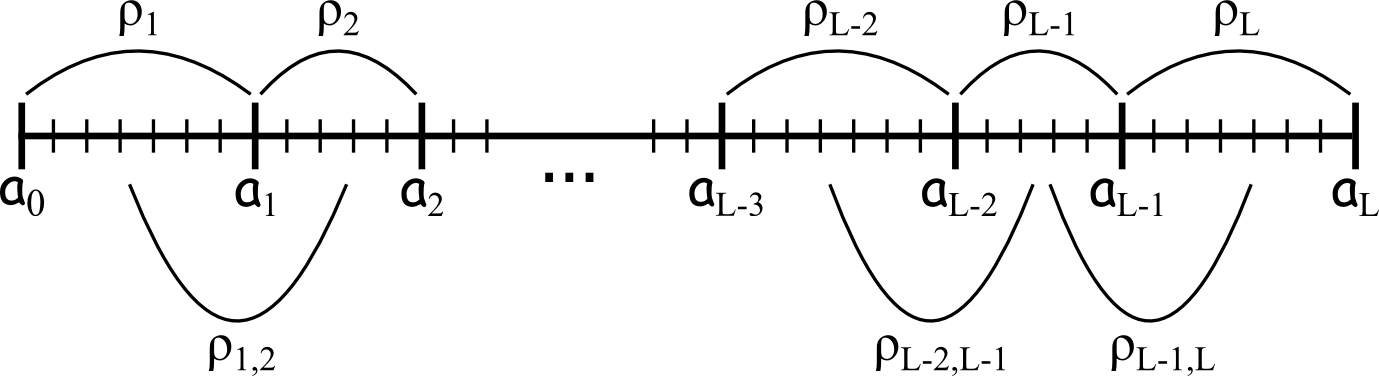
\includegraphics[width=8cm]{dinprog_modified.png}
	\caption{Модифицированная схема динамического программирования}
	\label{fig:2_2}
\end{figure}

На первом этапе рассматриваем 2 крайних правых части.
Последний узел $a_L$, как и ранее, считаем фиксированным.
Задаём приращения двум другим узлам и перебираем все сочетания значений $a_{L-1}^i$, $i = \overline{-m, m}$, $a_{L-2}^j$, $j = \overline{-m, m}$, то есть $(2m + 1)^2$ комбинаций.
Рассматриваемые 2 узла полностью определяют 2 крайних правых части, что позволяет вычислить значение суммы критериев 1 и 2 для каждой комбинации.
Для этого для всех индексов $i$, $j$ вычисляем оценки средних коэффициентов корреляции внутри каждой части $\rho_L^i$, $\rho_{L-1}^{j, i}$, а также оценку среднего коэффициента корреляции между частями $\rho_{L-1, L}^{j, i}$.
Тогда для 2 рассматриваемых частей $[a_{L-1} + 1; a_L]$, и $[a_{L-2} + 1; a_{L-1}]$ суммарные оценки средних коэффициентов корреляции (далее --- суммарные оценки) вычисляются по формуле $P_{L-1, L}^{j, i} = \rho_L^i + \rho_{L-1}^{j, i} + \rho_{L-1, L}^{j, i}$.
Всего получаем $(2m + 1)^2$ значений суммарных оценок, которые приписываем каждой из комбинаций значений узлов $a_{L-1}^i$ и $a_{L-2}^j$.

На втором этапе вводим в рассмотрение узел $a_{L-3}$, которому также придаём $2m + 1$ значений $a_{L-3}^l$, $l = \overline{-m, m}$.
Новый узел позволяет вычислить коэффициенты $\rho_{L-2}$ и $\rho_{L-2, L-1}$.
Эти коэффициенты зависят также от значений границ предыдущей части, то есть от значений $a_{L-1}^i$, $a_{L-2}^j$.
Используя эти значения и перебирая $(2m + 1)^3$ комбинаций по переменным $l$, $j$, $i$, вычисляем суммарные оценки $P_{L-2, L-1}^{l, j, i} = \rho_{L-2}^{l, j} + \rho_{L-2, L-1}^{l, j, i} + P_{L-1, L}^{j, i}$.
Выделяем значения, соответствующие узлам $a_{L-3}$ и $a_{L-2}$, то есть индексам $l$, $j$.
Каждой комбинации этих коэффициентов соответствуют $2m + 1$ значений узла $a_{L-1}$, то есть индекса $i$.
Возьмём по индексу $i$ максимум.
В итоге получим $(2m + 1)^2$ значений суммарного коэффициента, соответствующих узлам $a_{L-3}$ и $a_{L-2}$: $P_{L-2, L-1}^{l, j} = \max_{i} \{ P_{L-2, L-1}^{l, j, i} \}$.
Итого, результатом второго этапа являются $(2m + 1)^2$ комбинаций коэффициентов $a_{L-3}$ и $a_{L-2}$, каждой из которых присвоено значение суммарной оценки, оптимальное по всем возможным положениям узла $a_{L-1}$.

Действуя аналогично на предпоследнем этапе для узлов $a_1$ и $a_2$, получаем $(2m + 1)^2$ значений, каждому из которых присвоено значение суммарной оценки, оптимальное по всем возможным положениям узлов $a_3, \dots, a_{L-1}$: $P_{1, 2}^{l, j} = \max_{i} \{ P_{1, 2}^{l, j, i} \}$.
На последнем этапе добавляем узел $a_0$ и находим оптимальный вариант: $P_{1, 2} = \max_{l, j} \{ \rho_1^l + \rho_{1, 2}^{l, j} + P_{1, 2}^{l, j} \}$.

%3
После этого рассматривается алгоритм формирования эталонов на основе метода главных компонент.
Оптимальный эталон формируется путём разложения усреднённого эталона на главные компоненты и дальнейшей оптимизацией коэффициентов разложения на обучающей выборке с помощью метода покоординатного спуска.
Полученный в результате оптимизации эталон может быть применён в любых алгоритмах, которые используют сравнение с эталоном.

Пусть имеется $M$ параметрических портретов различных реализаций одного слова $X = \{x_{ij}(k)\}$, $k = 1, 2, \dots, M$; $i = 1, 2, \dots, N_t$; $j = 1, 2, \dots, N_f$.
Преобразуем для каждого $k$ матричный портрет в одномерный массив с числом элементов $i = 1, 2, \dots, P$, $P = N_f N_t$ и объединим эти $M$ векторов в матрицу размерности $P \times M$:

\begin{equation}
X = \begin{bmatrix} x_1 & x_2 & \dots & x_M \end{bmatrix} = 
\begin{bmatrix}
	x_{11} & x_{12} & \dots  & x_{1M} \\
	x_{21} & x_{22} & \dots  & x_{2M} \\ 
	\vdots & \vdots & \ddots & \vdots \\
	x_{P1} & x_{P2} & \dots  & x_{PM} \\
\end{bmatrix}.
\end{equation}

Матрица корреляционных моментов равна $K_x = X^T X$ и является симметричной.
Для неё можно вычислить $M$ собственных чисел $\lambda_1, \lambda_2, \dots, \lambda_M$ (упорядочены по убыванию) и соответствующие им собственные векторы $l_1, l_2, \dots, l_M$.
Первая главная компонента $a_1$ определяется как линейная комбинация исходных векторов $x_1, x_2, \dots, x_M$, взятых с коэффициентами, равными элементам собственного вектора $l_1^T= [l_{11} l_{21} \dots l_{M1}]$.
Аналогично вычисляются остальные главные компоненты.
Смысл применения главных компонент состоит в том, что поведение системы определяется в основном несколькими первыми главными компонентами $a_j$, $j = 1, 2, \dots, M'$, $M' < M$.
Это позволяет уменьшить размерность задачи и рассматривать $M'$ главных компонент вместо $M$ исходных векторов.

Далее, представим эталон как линейную комбинацию $M'$ главных компонент и постоянной составляющей с некоторыми коэффициентами: $E_{syn} = k_0 a_0 + k_1 a_1 + \dots + k_{M'} a_{M'}$.
Задача поиска оптимального эталона сводится к подбору таких коэффициентов $k_0, \dots, k_{M'}$, которые будут удовлетворять критерию: значение Z-коэффициента корреляции $\rightarrow \max$.
Для случая распознавания 3 слов суммарный критерий описывается формулой $F = \Delta Z^{low}_{1} + \Delta Z^{low}_{2} + \Delta Z^{low}_{3}$, где $\Delta Z^{low}_{i} = \min(\Delta Z_{ij}, \Delta Z_{ik})$, $i \ne j$, $i \ne k$, $j \ne k$, а $\Delta Z_{ij}$ --- это разница Z-преобразований Фишера коэффициентов корреляций $i$-го эталона с распознаваемым $i$-м словом и $j$-го эталона с распознаваемым $i$-м словом. 

Также можно дополнительно штрафовать за неправильное распознавание слова, что эквивалентно штрафу за значения $Z^{low}_{i}$ меньше нуля: $F = \Delta Z^{*low}_{1} + \Delta Z^{*low}_{2} + \Delta Z^{*low}_{3}$, где $\alpha$ --- это некоторое положительное число и

\begin{equation}
\Delta Z^{*low}_{i} = \left\{
\begin{array}{ll}
	\Delta Z^{low}_{i}, \qquad\qquad\qquad \Delta Z^{low}_{i} \ge 0,\\
	\Delta Z^{low}_{i} - \alpha (\Delta Z^{low}_{i})^2, \Delta Z^{low}_{i} < 0.
\end{array}
\right.
\end{equation}

Подбор коэффициентов на каждой итерации производится для каждого слова по очереди, при этом коэффициенты разложения двух других слов остаются неизменными.

%4
Затем рассматривается разработка алгоритма формирования эталонов на основе полиномов Чебышёва.
Пусть у нас есть параметрический портрет $X$, который содержит $N_f$ частотных полос и $N_t$ временных интервалов.
Данный параметрический портрет помимо самого речевого сигнала содержит ещё и неинформативные сигналы, обусловленные особенностями речи определённого диктора и шумами.
Использование полиномов Чебышёва поможет выделить только информативную часть, решив при этом сразу несколько задач.
Во-первых, позволит уменьшить размерность параметрического портрета без существенной потери информативности, что упростит его хранение и ускорит обработку.
Во-вторых, выделение только самого речевого сигнала может повысить качество распознавания.
Сжатие можно производить по частотным полосам, по временным интервалам и по обоим измерениям одновременно.
Также возможно использование полиномов Чебышёва не только для записей слов, но и для эталонов.

%5
В конце рассмотрена разработка алгоритмов распознавания команд с использованием нескольких дикторов на основе формулы Байеса и метода комитетов.
Для обеспечения дикторонезависимости распознавания следует увеличивать разнообразие речевого материала в обучающей базе, например, за счёт применения нескольких эталонов, сформированных по записям разных дикторов.
В данных алгоритмах для улучшения результатов распознавания могут быть применены подстройка по времени и оптимизированные эталоны, а также для ускорения работы может быть использовано сжатие используемых параметрических портретов.

Первый алгоритм использует формулу Байеса.
В этом случае на основе обучающей выборки формируются априорные условные вероятности возможных вариантов распознавания слов, используемые для расчёта апостериорных вероятностей, что позволяет улучшить оценки и, как следствие, качество распознавания при невозможности выбора состава команд.

Пусть имеются гипотезы $H_1, \dots, H_M$, соответствующие полной группе несовместных событий с априорными вероятностями $P(H_1), \dots, P(H_M)$.
Пусть в результате распознавания по одному эталону произошло событие $A_k$, то есть принята гипотеза $H_k$.
Тогда по формуле Байеса условная апостериорная вероятность каждой гипотезы при условии, что произошло событие $A_k$, равна $P(H_i|A_k) = P(H_i) P(A_k|H_i) / \sum_{j=1}^M P(H_j) P(A_k|H_j)$, $i = 1, \dots, M$.
Для использования данной формулы необходимо определить априорные вероятности гипотез $P(H_1), \dots, P(H_M)$ и получить для всех событий $A_k$ оценки априорных вероятностей события $P(A_k|H_i)$, $k = 1, \dots, M$.
Изначально все априорные вероятности можно принимать равновероятными $P(H_i) = 1/M$ или использовать апостериорные вероятности, полученные на предыдущем этапе для случая многоэтапной процедуры распознавания.

Необходимо также получить оценки априорных условных вероятностей $P(A_k|H_i)$.
Для этого необходимо использовать обучающую выборку: $P(A_k|H_i) = e_{ki} / E$, где $e_{ki}$ --- число событий $A_k$, при условии, что верна гипотеза $H_i$.
Для случая $L$ эталонов в формуле Байеса необходимо изменить только количество индексов: $P(H_i|A_{k_1 \dots k_L}) = P(H_i) P(A_{k_1 \dots k_L}|H_i) / \sum_{j=1}^M P(H_j) P(A_{k_1 \dots k_L}|H_j)$.

Также дополнительная возможность для улучшения распознавания заключается в использовании значений меры близости $Z$ как показателей качества распознавания.
Введём характеристику качества распознавания $\Delta Z = Z_{\max} - Z_{\max - 1}$, где $Z_{\max}$ --- максимальное значением меры близости $Z$ между параметрическими портретами распознаваемого слова и всеми $M$ субэталонами, а $Z_{\max - 1}$ --- значение, ближайшее к максимальному.
Можно принять, что качество распознавания прямо пропорционально значению показателя $\Delta Z$.
Тогда формула для одного эталона с учётом качества распознавания будет следующей:
\begin{equation}
P(H_i|A_k^{\Delta Z}) = \frac{P(H_i) P(A_k|H_i) P(\Delta Z|H_i)}{\sum_{j=1}^M P(H_j) P(A_k|H_j) P(\Delta Z|H_j)}.
\end{equation}
Для случая нескольких эталонов формула определяется аналогично.

Второй алгоритм основан на методе комитетов и заключается в независимом распознавании команд разными эталонами.
На вход системы распознавания поступает неизвестное слово, которое последовательно распознаётся при помощи $L$ эталонов, то есть вычисляются значения скалярной меры близости $Z_i^j$, где $j$ --- номер эталона, $j = 1, 2, \dots, L$, а $i$ --- номер субэталона, $i = 1, 2, \dots, M$.
Предлагается для каждого $j$-го эталона сформировать коэффициенты $r_i^j = Z_i^j \Delta Z^j/ p_i^j$, где $p_i^j$ --- место в рейтинге субэталонов.

Формула исходит из очевидных эвристических соображений.
Действительно, <<правильный>> субэталон, то есть соответствующий распознаваемому слову, должен иметь наибольшую меру близости $Z_i^j$, наибольшее удаление $\Delta Z^j$ от всех остальных субэталонов и наименьшее по порядковому номеру, то есть первое, место в рейтинге.
Поэтому для <<правильного>> субэталона коэффициент $r_i^j$ максимален. 
Далее баллы, полученные по всем эталонам, суммируются и формируют итоговую оценку, на основе которой определяется результат распознания.

%============================================================================================================================

%1
\textbf{Третий раздел} посвящён экспериментальному оцениванию характеристик распознавания предложенных алгоритмов.
В начале описывается тестовая база речевых данных.
В работе используется 2 основных набора слов и 1 набор фраз.
Первый набор представляет собой записи 3 слов, произнесённых 13 дикторами, каждый диктор произносит около 50 реализаций каждого слова.
Второй набор данных содержит 20 слов, произнесённых 9 дикторами, при этом каждый диктор произносит каждое слово по 30 раз.
Последний набор состоит из 11 фраз, произнесённых 7 дикторами, при этом каждый диктор произносит каждую фразу по 30 раз.

Также используются записи с фоновым шумом и с шумом в наушниках.
Шум в наушниках реализуется следующим образом.
Диктор надевает наушники, в которые подаётся шум заданной громкости, при этом диктор плохо слышит свой голос, поскольку к наушникам не подключена обратная связь.
Это используется для того, чтобы в экспериментальных условиях проверить степень изменения речи диктора в зависимости от уровня шума.

После этого была проведена проверка гипотез о нормальности распределения отклонения элементов параметрических портретов слов от эталона, а также показаны результаты расчётов длительности слов, их энергии и частоты.
Для проверки был использован первый набор данных, состоящий из записей 3 слов без шума.
Результаты показывают, что происходит увеличение доли проверок, подтверждающих нормальность по критерию Пирсона, с 30~\% для случая некорректированных по амплитуде слов до 86~\% проверок для слов, корректированных по амплитуде.
По результатам статистической проверки можно сделать вывод, что после выравнивания слов по амплитуде входной сигнал удовлетворяет критерию нормальности.
Поэтому дальнейшее использование алгоритмов, требующих нормальности входных данных, обосновано.

%2
Далее описываются результаты экспериментов по разделению слов на однородные части.
В качестве эталона принимался результат <<ручного>> разбиения, при котором границы частей определялись по результатам прослушивания и визуального анализа спектрограмм записи слова.
На нескольких примерах было проведено сравнение метода полного перебора и рассмотренных выше алгоритмов динамического программирования, которое показало высокую точностью совпадения результатов.
Поэтому в дальнейшем использовался только метод динамического программирования, который позволяет проводить разбиение записи одного слова меньше чем за секунду.
Рассматривалось разбиение слов на 3--7 частей, при этом одна часть могла содержать от 2 до 25 интервалов.
Диапазон варьирования границ частей принимался от минус 5 до плюс 5 элементарных интервалов от начального положения каждой границы.
Обработка каждого слова выполнялась несколько раз для разных априорных значений положения границ.
При этом практически отсутствовала зависимость результатов от априорных оценок при условии, что оптимальное значение находилось в области поиска. 

Один из рассмотренных примеров --- это слово <<тысяча>>.
В нём можно выделить 6 хорошо различимых звуков, по одному на каждую букву слова, что хорошо видно на рисунке \ref{fig:3_1} и в таблице \ref{tab:3_1}.
\begin{figure}[h]
	\centering
	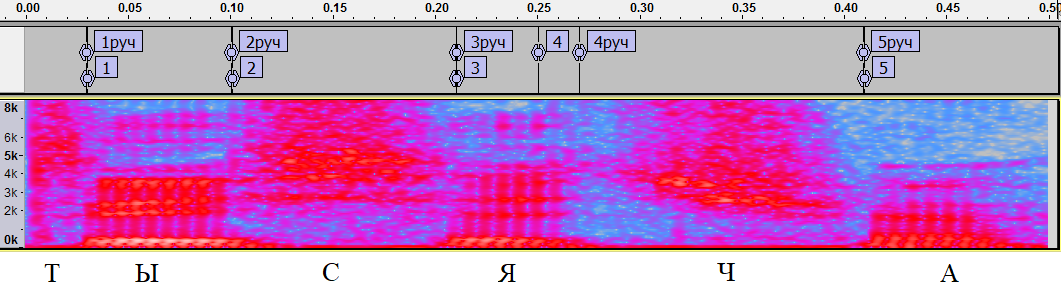
\includegraphics[width=0.9\textwidth]{word_1000.png}
	\caption{Результаты разбиения слова <<тысяча>>}
	\label{fig:3_1}
\end{figure}

\begin{table}[h]
	\centering
	\caption{Границы частей для разных критериев, слово <<тысяча>>}
	\label{tab:3_1}
	\begin{tabular}{| l | c | c | c | c | c | c |}
		\hline
		\multirow{2}{*}{Функционал} & \multicolumn{5}{c|}{Границы частей, с} & Значение \\
		\hhline{~-----~} & \phantom{00}1\phantom{00} & \phantom{00}2\phantom{00} & \phantom{00}3\phantom{00} & \phantom{00}4\phantom{00} & \phantom{00}5\phantom{00} & \phantom{0}функционала\phantom{0} \\
		\hline
		$J_{1}$		& 0.03 & 0.10 & 0.21 & 0.25 & 0.41 & 0.75 \\
		$J_{2}$		& 0.03 & 0.10 & 0.21 & 0.24 & 0.41 & 0.01 \\
		$J_{3}$		& 0.03 & 0.10 & 0.21 & 0.25 & 0.41 & 0.13 \\
		$J_{12}$	& 0.03 & 0.10 & 0.21 & 0.24 & 0.41 & 0.74 \\
		$J_{123}$	& 0.03 & 0.10 & 0.21 & 0.24 & 0.41 & 0.60 \\
		\hline
		Вручную		& 0.03 & 0.10 & 0.21 & 0.27 & 0.41 & --- \\
		\hline
	\end{tabular}
\end{table}

Аналогичные разбиения проводились и для других 5 слов.
Анализ показывает достаточно хорошее совпадение границ, найденных автоматически, и эталонных границ, полученных в ручном режиме обработки.
Проведённая обработка показывает также, что результаты, полученные при помощи различных критериев, близки между собой, особенно в тех случаях, когда однородные части содержат отдельные звуки, что соответствует допущениям, принятым при формировании критериев.
Таким образом, проведённые эксперименты подтверждают работоспособность предложенных алгоритмов автоматического разбиения слов на фонетически однородные части.

%3
Затем приводятся результаты эксперимента с получением оптимального эталона через метод главных компонент.
Здесь тестирование алгоритма производится на примере простой задачи распознавания 3 слов, которые произносятся 10 различными дикторами в условиях без шума и 4 дикторами в условиях с шумом в наушниках (80 дБ и 90 дБ).

Вначале проводится проверка эффективности выделения главных компонент.
Было показано, что первая главная компонента несёт в себе порядка 98~\% имеющейся информации, первые 3 главных компоненты --- 99~\%, а при 6 главных компонентах доля достигает 99.5~\%.

Результаты применения оптимизированного на обучающей выборке эталона, приведённые в таблице \ref{tab:3_2}, показывают улучшение при распознавании реализаций не только для слов диктора, используемого в обучающей выборке, но также и для других дикторов, не входящих в обучающую выборку.
Процент ошибок для 1200 записей трёх слов до оптимизации равнялся 5~\%, а после оптимизации уменьшился до 1.25~\%.

\begin{table}[h]
	\centering
	\caption{Число ошибок распознавания слов с шумом в наушниках 80 дБ на обычном (1) и оптимизированном (2) эталонах и с шумом в наушниках 90 дБ на обычном (3) и оптимизированном (4) эталонах}
	\label{tab:3_2}
	\begin{tabular}{| c | c | c | c | c | c |}
		\hline
		\phantom{000}Диктор\phantom{000}& Слово & \phantom{00} (1) \phantom{00} & \phantom{00} (2) \phantom{00} & \phantom{00} (3) \phantom{00} & \phantom{00} (4) \phantom{00} \\
		\hline
				& пилотаж	& 6 & 0 & 7 & 0 \\
		Б-ак	& масштаб	& 0 & 0 & 0 & 0 \\
				& навигация & 0 & 8 & 0 & 1 \\
		\hline
				& пилотаж	& 3 & 0 & 3 & 0 \\
		Г-ов	& масштаб   & 0 & 0 & 0 & 0 \\
				& навигация & 0 & 0 & 0 & 2 \\
		\hline
				& пилотаж	& 8 & 0 & 12& 0 \\
		Н-ов	& масштаб   & 0 & 0 & 0 & 0 \\
				& навигация & 0 & 0 & 0 & 0 \\
		\hline
				& пилотаж	& 9 & 0 & 4 & 0 \\
		Ф-ев	& масштаб   & 0 & 0 & 0 & 0 \\
				& навигация & 0 & 0 & 8 & 4 \\
		\hline
		\multicolumn{2}{|c|}{Суммарные результаты} & \multicolumn{2}{c|}{\textbf{26} $\quad\longrightarrow\quad$ \textbf{8}} & \multicolumn{2}{c|}{\textbf{34} $\quad\longrightarrow\quad$ \textbf{7}} \\
		\hline
	\end{tabular}
\end{table}

Также было протестировано использование ограниченного числа реализаций слов, используемых при построении оптимального эталона, и заранее заданного количества итераций оптимизации.
Эксперимент показал, что достаточно использовать только 1 реализацию слова и проводить всего 10 итераций для получения оптимального эталона, что заметно сокращает время работы программы.

%4
После этого описываются результаты экспериментов, связанных с аппроксимацией полиномами Чебышёва.
Эксперимент проводился на параметрических портретах 20 слов, произнесённых 9 дикторами.
Изначальные параметрические портреты содержали 35 частотных полос и 48 временных интервалов.
Наиболее оптимальным в плане уменьшения размера параметрического портрета является одновременное сжатие и по частотным полосам, и по временным интервалам.

При использовании исходных записей без сжатия было получено 1.6~\% ошибок.
При использовании 18 полиномов в разложении по обоим измерениям получается 1.8~\%, для 14 полиномов --- 1.9~\% ошибок и 2.0~\% ошибок для 12 полиномов.
Это позволяет уменьшить число элементов в параметрическом портрете в 5--10 раз.
Полное совпадение количества ошибок достигается при очень большом числе полиномов, позволяя лишь незначительно уменьшить размеры параметрического портрета.

%5
В конце показаны результаты распознаваний алгоритмами на основе формулы Байеса и метода комитетов.
Проверка алгоритмов распознавания была проведена на речевой базе, включающей 20 слов для 8 дикторов.
Формирование эталона во всех экспериментах проводилось по речевому материалу диктора, который не включался в распознаваемые записи, то есть был реализован дикторонезависимый вариант распознавания.

Результаты экспериментов представлены ниже в таблице \ref{tab:3_4}.
В первом столбце указан вариант распознавания: по одному эталону, который формировался по записям одного диктора, с точностью до единственного слова и с точностью до группы из 2 или 3 слов.
\begin{table}[h]
	\centering
	\caption{Процент ошибок при распознавании по 7 эталонам}
	\label{tab:3_4}
	\begin{tabular}{| l | c | c | c | c | c | c | c | c | c |}
		\hline
		Вариант & \multicolumn{8}{c|}{Порядковый номер диктора} & Среднее \\
		\hhline{~--------}
		теста & 1 & 2 & 3 & 4 & 5 & 6 & 7 & 8 & \phantom{0}значение\phantom{0} \\
		\hline
		\hline
		1 эталон	& 5.3 & 9.3 & 15  & 8.0 & 5.0 & 11  & 7.0 & 6.7 & \textbf{8.42} \\
		\hline
		\multicolumn{10}{|c|}{алгоритм на основе формулы Байеса} \\
		\hline
		до 1 слова	& 4.8 & 7.3 & 7.3 & 4.8 & 6.5 & 6.3 & 4.7 & 3.2 & \textbf{5.62} \\
		до 2 слов	& 2.7 & 4.8 & 3.8 & 2.2 & 2.5 & 2.7 & 2.2 & 0.8 & 2.71 \\
		до 3 слов	& 2.5 & 3.5 & 3.0 & 1.8 & 2.2 & 2.2 & 2.0 & 0.7 & 2.23 \\
		\hline
		\multicolumn{10}{|c|}{алгоритм на основе метода комитетов} \\
		\hline
		до 1 слова	& 4.5 & 7.3 & 7.2 & 4.8 & 4.5 & 6.7 & 4.8 & 2.8 & \textbf{5.33} \\
		до 2 слов	& 0.7 & 3.3 & 2.8 & 1.3 & 1.7 & 2.7 & 1.0 & 1.3 & 1.85 \\
		до 3 слов	& 0.5 & 2.5 & 1.0 & 0.5 & 1.3 & 1.7 & 0.5 & 0.5 & 1.06 \\
		\hline
		подстройка\phantom{00}	& 1.8 & 4.5 & 4.3 & 3.2 & 1.9 & 4.8 & 2.3 & 2.2 & \textbf{3.13} \\
		\hline
	\end{tabular}
\end{table}
Среднее количество ошибок при распознавании одним эталоном равно 8.42~\%.
Для эталонов по 7 дикторам получается заметное улучшение в 1.5--2 раза --- в этом случае средняя ошибка для алгоритма на основе формулы Байеса равна 5.62~\%, а для алгоритма на основе метода комитетов 5.33~\%.

Следует отметить, что более простой эвристический алгоритм на основе метода комитетов при тестировании показал несколько лучшие результаты, чем более сложный и математически обоснованный алгоритм, использующий формулу Байеса.
Наиболее вероятная причина заключается в том, что более сложный алгоритм оказывается чувствительным к погрешностям оценок априорных условных вероятностей и, следовательно, требует увеличения объёмов обучающих выборок.

Наилучший эффект, особенно для алгоритма на основе метода комитетов, достигается при переходе к группам из 2 и 3 слов, и такая возможность локализации распознаваемого слова имеет практический смысл.
Это позволяет существенно сократить время обработки за счёт перехода к иерархической процедуре распознавания: вначале быстродействующими алгоритмами выделяется малая группа, а затем в рамках группы проводится поиск алгоритмами, более затратными по времени, например, подстройкой по длительности или сравнением с эталонами <<чужих>> слов.
Результат применения такого подхода для алгоритма на основе метода комитетов снижает число ошибок до 3.13~\%, что в 2.7 раз меньше изначального результата при распознавании эталоном одного диктора.

%============================================================================================================================

В \textbf{четвёртом разделе} приведено описание разработки алгоритмов автоматического распознавания речевых команд на основе свёрточных нейронных сетей глубокого обучения.
В распознавании использовались параметрические портреты с 18 частотными полосами и 25 временными интервалами.
В данном случае для уменьшения размерности параметрических портретов может быть использован метод сжатия портретов на основе полиномов Чебышёва.
Также для всех портретов из обучающей выборки может быть применено разбиение на однородные части и выравнивание найденных частей относительно друг друга для каждого слова.

Вначале были проведены оценки работоспособности традиционных сетей типа одно- и двухслойных персептронов в задаче распознавания речевых команд.
Они показали неудовлетворительные результаты, с количеством ошибок в несколько раз больше чем в ранее приведённых методах.

% без шума
После этого были апробированы нейронные сети глубокого обучения.
Для них была выбрана оптимальная архитектура сети, имеющая по 2 слоя свёртки и подвыборки, за которыми идут 3 полносвязных слоя.
Между полностью связанными слоями производится регуляризация, состоящая в случайном выбрасывании определённого количества нейронов в процессе обучения.
Такой приём предотвращает переобучение и повышает стабильность результатов.
Структура сети показана на рисунке \ref{fig:4_1}.

\begin{figure}[h]
	\centering
	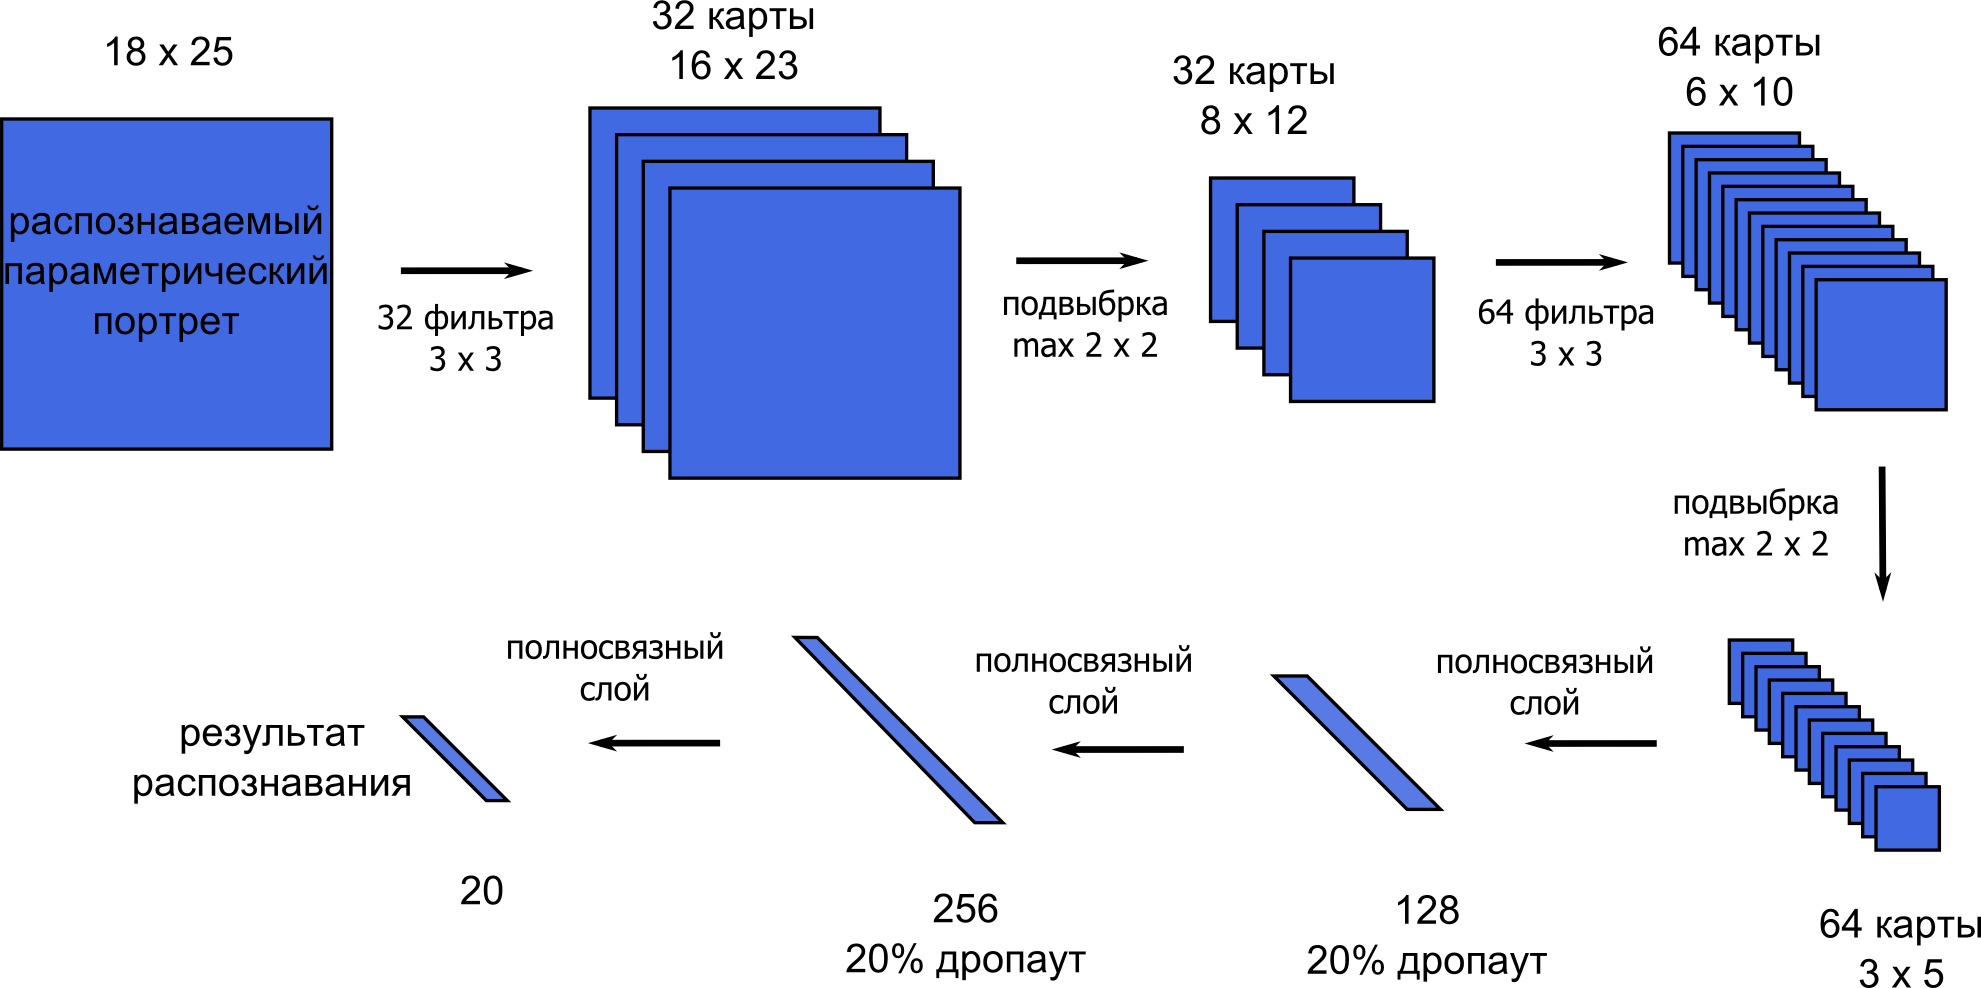
\includegraphics[width=1.0\textwidth]{cnn_my.png}
	\caption{Архитектура используемой свёрточной нейронной сети}
	\label{fig:4_1}
\end{figure}

В таблице \ref{tab:4_1} приведены суммарные результаты распознавания записей без шума при обучении на различном числе дикторов.
\begin{table}[h]
	\centering
	\caption{Результаты распознаваний слов и фраз на обучающих наборах из различного количества дикторов для случая записей без шума}
	\label{tab:4_1}
	\begin{tabular}{| l | c | c | c | c | c | c | c |}
		\hline
		Процент\phantom{0} & \multicolumn{7}{c|}{Количество дикторов в обучающей выборке} \\
		\hhline{~-------}
		ошибок & \phantom{00}1 \phantom{00} & \phantom{00}2 \phantom{00} & \phantom{00}3 \phantom{00} & \phantom{00}4 \phantom{00} & \phantom{00}5 \phantom{00} & \phantom{00}6 \phantom{00} & \phantom{00}7 \phantom{00} \\
		\hline
		Слова		& 5.9 & 2.4 & 1.7 & 1.2 & 1.0 & 0.8 & 0.6 \\
		\hline
		Фразы 		& 18.0 & 11.4 & 6.9 & 5.4 & 4.8 & 4.2 & --- \\
		\hline
	\end{tabular}
\end{table}

Из результатов можно сделать вывод, что процент ошибок стабильно снижается при увеличении количества дикторов в обучающей базе.
Большее число дикторов позволяет избавиться от дикторозависимости, что положительно сказывается на качестве распознавания.

% с шумом
На рисунке \ref{fig:cnn_self_noise} представлены усреднённые результаты распознаваний слов и фраз в условиях различных уровней шума при обучении на том же дикторе.
Записи каждого диктора разбивались на 2 части --- на первой части обучалась свёрточная нейронная сеть, а вторая часть использовалась в качестве тестовой выборки.
\begin{figure}[h]
	\centering
	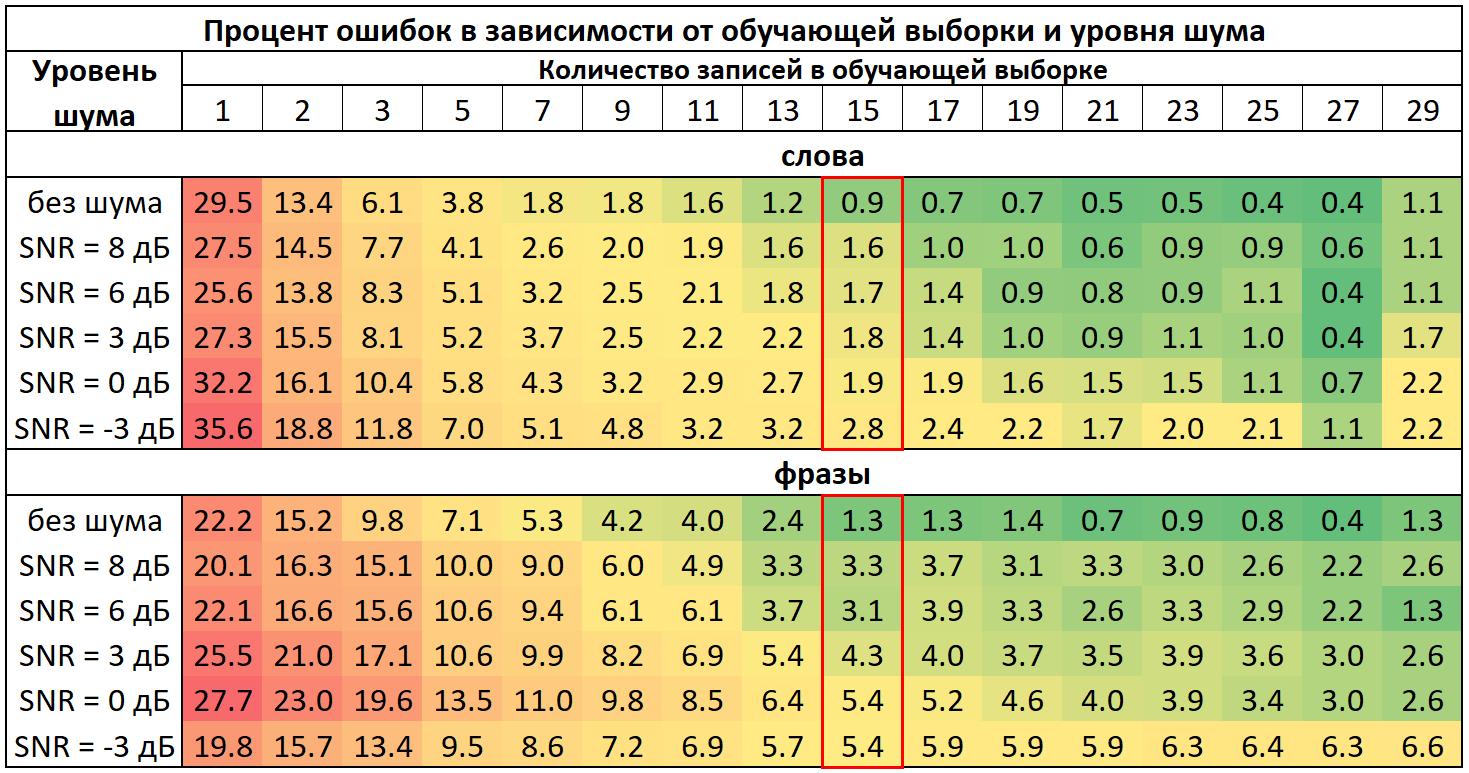
\includegraphics[width=1.0\textwidth]{cnn_self_noise.png}
	\caption{Результаты распознаваний при различных уровнях шума при обучении на том же дикторе, указан процент ошибок распознаваний}
	\label{fig:cnn_self_noise}
\end{figure}

По результатам видно, что при обучении на всего лишь 15 записях каждого слова получается 0.9~\% ошибок для слов и 1.3~\% ошибок для фраз.
При добавлении шума процент ошибок незначительно возрастает.
Например, при отношении сигнал/шум равному 0 дБ, процент ошибок возрастает до 1.9~\% для слов и до 5.4~\% для фраз.

В таблице \ref{tab:4_2} приведены суммарные результаты распознавания записей с шумом при обучении на различном числе дикторов и различном количестве наложенных шумов.
\begin{table}[h]
	\centering
	\caption{Результаты распознавания по <<чужому>> диктору при обучении на различном числе дикторов для записей слов и фраз с шумом}
	\label{tab:4_2}
	\begin{tabular}{| l | c | c | c | c | c | c | c |}
		\hline
		\multicolumn{1}{|c|}{---} & \multicolumn{7}{c|}{Слова} \\
		\hline
		число дикторов\phantom{0000} & \multicolumn{2}{c|}{1} & \multicolumn{2}{c|}{3} & \multicolumn{2}{c|}{7} & --- \\
		\hline
		число шумов & \phantom{0} 1 \phantom{0} & \phantom{0} 7 \phantom{0} & \phantom{0} 1 \phantom{0} & \phantom{0} 3 \phantom{0} & 1 & 3 & --- \\
		\hline
		процент ошибок & 9.7 & 8.2 & 2.8 & 2.5 & 1.2 & 1.1 & --- \\
		\hline
		\multicolumn{1}{|c|}{---} & \multicolumn{7}{c|}{Фразы} \\
		\hline
		число дикторов & \multicolumn{3}{c|}{1} & \multicolumn{2}{c|}{3} & \multicolumn{2}{c|}{6} \\
		\hline
		число шумов & 1 & 5 & 10 & 1 & \phantom{0} 5 \phantom{0} & \phantom{0} 1 \phantom{0} & \phantom{0} 2 \phantom{0} \\
		\hline
		процент ошибок & 22.4 & 21.1 & 20.8 & 11.5 & 10.4 & 8.4 & 7.0 \\
		\hline
	\end{tabular}
\end{table}

Из результатов можно сделать вывод, что процент ошибок стабильно снижается при увеличении количества дикторов в обучающей базе.
Также можно сделать вывод, что увеличение количества накладываемых шумов приводит к уменьшению числа ошибок, но этот эффект от увеличения обучающей базы выражен менее заметно.
Большое количество шумов в обучающей выборке уменьшает эффект переобучения для определённого типа шума, что уменьшает число ошибок при распознавании записей с другим шумом.

% добавление своих записей
В конце проверялось, как изменится качество распознавания команд при обучении по фразам чужого диктора с добавлением небольшого числа записей своего диктора.
При этом, это будут разные реализации команд, то есть добавленные к обучающей выборке записи исключаются из тестовой выборки.
Таким образом, можно учесть некоторые индивидуальные особенности распознаваемого диктора при добавлении лишь небольшого числа фраз, что достаточно несложно реализуется на практике.

В таблице \ref{tab:4_3} приведены результаты распознавания в эксперименте для различных конфигураций.
\begin{table}[h]
	\centering
	\caption{Результаты распознавания при добавлении фраз к обучающей выборке, состоящей из записей нескольких дикторов}
	\label{tab:4_3}
	\begin{tabular}{| l | c | c | c | c | c | c | c |}
		\hline
		Число & \multicolumn{7}{c|}{Процент ошибок при заданном числе добавленных записей} \\
		\hhline{~-------}
		дикторов & \phantom{00}0\phantom{00} & \phantom{00}1\phantom{00} & \phantom{00}2\phantom{00} & \phantom{00}3\phantom{00} & \phantom{00}5\phantom{00} & \phantom{00}10\phantom{00} & \phantom{00}15\phantom{00} \\
		\hline
		1 		 & 18.0 & 8.8 & 7.2 & 6.4 & 5.2 & 3.7 & 1.9 \\
		2 		 & 11.4 & 7.1 & 6.1 & 5.2 & 4.8 & 3.6 & 1.6 \\
		3 		 &  6.9 & 5.2 & 4.8 & 4.3 & 3.8 & 3.1 & 1.2 \\
		4 		 &  5.4 & 4.6 & 3.7 & 3.7 & 3.2 & 2.7 & 1.1 \\
		5 		 &  4.8 & 4.3 & 4.1 & 3.9 & 3.5 & 2.7 & 1.2 \\
		6 		 &  4.2 & 3.9 & 3.8 & 3.7 & 3.2 & 2.9 & 1.2 \\
		\hline
	\end{tabular}
\end{table}

Как видно из результатов, при добавлении всего по 1 реализации каждой из фраз <<своего>> диктора в обучающую выборку ошибка распознавания уменьшается больше чем в 2 раза с 18.6 до 8.8~\%.
Дальнейшее добавление записей снижает ошибку, но величина снижения уже не такая большая.
Также, эффект от добавленных записей тем больше, чем меньше дикторов использовано в обучающей выборке.

В \underline{\textbf{заключении}} приведены основные результаты работы, которые состоят в следующем:
%% Согласно ГОСТ Р 7.0.11-2011:
%% 5.3.3 В заключении диссертации излагают итоги выполненного исследования, рекомендации, перспективы дальнейшей разработки темы.
%% 9.2.3 В заключении автореферата диссертации излагают итоги данного исследования, рекомендации и перспективы дальнейшей разработки темы.

\begin{enumerate}[label={\arabic*)}]
	\item Разработан автоматический алгоритм разбиения слов на однородные части, в основе которого нахождение положения границ частей производится с помощью многопараметрической оптимизации.
	Сформулированы критерии, реализующие принцип максимизации меры сходства фонетического материала внутри части и меры различия между соседними частями. 
	Для численного решения задачи с высоким быстродействием предложены алгоритмы, основанные на методе динамического программирования.
	Эксперименты, проведённые на примерах нескольких слов русского языка, подтвердили работоспособность предложенного подхода и правомерность принятых допущений.
	\item Разработан алгоритм улучшения качества эталона, основанный на выделении и оптимизации главных компонент.
	Эталон, полученный с помощью оптимизации коэффициентов при главных компонентах, показал значительно меньшее число ошибок при распознавании большинства записей.
	Общее количество ошибок для записей слов с шумом в наушниках до оптимизации равнялось 5~\%, а после оптимизации уменьшилось до 1.25~\%.
	Также был сделан вывод о том, что для получения приемлемых результатов достаточно использовать только одну реализацию слова и проводить всего 10 итераций при получении оптимального эталона, что заметно сокращает время работы программы.
	\item Изучены способы и разработаны алгоритмы сжатия информации о параметрическом портрете с помощью применения полиномов Чебышёва.
	Эксперименты показали, что сжатие может происходить как отдельно по частотам и по времени, так и по обоим измерениям одновременно.
	В последнем случае можно сократить место для хранения параметрического портрета в 5--10 раз практически без ухудшения качества распознавания.	
	\item Разработаны алгоритмы на основе формулы Байеса и метода комитетов, позволяющие заметно уменьшить количество ошибок распознавания при использовании нескольких эталонов.
	Первый алгоритм использует оценки априорных вероятностей, определяемые по обучающей выборке, и рассчитывает апостериорные вероятности формулы Байеса, а второй является модификацией известного метода комитетов.
	Выявленная в ходе тестирования возможность локализации распознаваемого слова с точностью до малой группы позволяет повышать быстродействие систем распознавания на основе иерархических процедур, в которых последовательно применяются алгоритмы распознавания разных видов.
	Работоспособность обоих разработанных алгоритмов подтверждается результатами тестирования.
	При использовании 7 эталонов, полученных по записям различных дикторов, достигается заметное снижение процента ошибок в 1.5--2 раза --- средняя ошибка для алгоритма на основе формулы Байеса снизилась с 8.42 до 5.62~\%, а для алгоритма на основе метода комитетов до 5.3 и до 3.13~\% при использовании подстройки по времени.
	\item Изучены и модифицированы алгоритмы распознавания речевых команд на основе искусственных нейронных сетей глубокого обучения.
	Наилучшие результаты показала архитектура нейронных сетей CNN с двумя слоями свёртки и тремя полностью связанными слоями.
	При обучении на словаре из 20 слов без шума на 7 дикторах средняя величина ошибки при распознавании <<чужих>> дикторов равна 0.6~\%.
	При обучении в той же конфигурации, но на записях с добавленным шумом, величина ошибки достигает для <<чужого>> диктора 1.1~\%.
	Эксперименты по распознаванию фраз при использовании обучающей выборки из записей 6 дикторов показали 4.2~\% ошибок для случая без шума и 7.0~\% для записей с шумом.
	Получены положительные результаты в дикторозависимом варианте распознавания без шума и в условиях шума при использовании небольшого числа записей каждой команды в обучающей выборке.
	Также получено значительное улучшение качества распознавания при добавлении всего нескольких реализаций каждой из речевых команд <<своего>> диктора в обучающую выборку, состоящую из записей <<чужих>> дикторов.
	При использовании нейронных сетей CNN количество ошибок является заметно более низким, чем для других алгоритмов, единственный замеченный недостаток --- это длительное время обучения нейронной сети.
\end{enumerate}


% При использовании пакета \verb!biblatex! список публикаций автора по теме диссертации формируется в разделе <<\publications>>\ файла \verb!common/characteristic.tex!  при помощи команды \verb!\nocite!

\begin{center}
	{\fontsize{11}{13}\selectfont \textbf{Публикации автора по теме диссертации}}
\end{center} 

\ifdefmacro{\microtypesetup}{\microtypesetup{protrusion=false}}{} % не рекомендуется применять пакет микротипографики к автоматически генерируемому списку литературы
\urlstyle{rm}                               % ссылки URL обычным шрифтом
\ifnumequal{\value{bibliosel}}{0}{% Встроенная реализация с загрузкой файла через движок bibtex8
	\renewcommand{\bibname}{\large \bibtitleauthor}
	\nocite{*}
	\insertbiblioauthor           % Подключаем Bib-базы
	%\insertbiblioexternal   % !!! bibtex не умеет работать с несколькими библиографиями !!!
}{% Реализация пакетом biblatex через движок biber
	% Цитирования.
	%  * Порядок перечисления определяет порядок в библиографии (только внутри подраздела, если `\insertbiblioauthorgrouped`).
	%  * Если не соблюдать порядок "как для \printbibliography", нумерация в `\insertbiblioauthor` будет кривой.
	%  * Если цитировать каждый источник отдельной командой --- найти некоторые ошибки будет проще.
	
	\ifnumgreater{\value{usefootcite}}{0}{
		\begin{refcontext}[labelprefix={}]
			\ifnum \value{bibgrouped}>0
			\insertbiblioauthorgrouped    % Вывод всех работ автора, сгруппированных по источникам
			\else
			\insertbiblioauthor      % Вывод всех работ автора
			\fi
		\end{refcontext}
	}{
		\ifnum \value{citeexternal}>0
		\begin{refcontext}[labelprefix=A]
			\ifnum \value{bibgrouped}>0
			\insertbiblioauthorgrouped    % Вывод всех работ автора, сгруппированных по источникам
			\else
			\insertbiblioauthor      % Вывод всех работ автора
			\fi
		\end{refcontext}
		\else
		\ifnum \value{bibgrouped}>0
		\insertbiblioauthorgrouped    % Вывод всех работ автора, сгруппированных по источникам
		\else
		\insertbiblioauthor      % Вывод всех работ автора
		\fi
		\fi
		%  \insertbiblioauthorimportant  % Вывод наиболее значимых работ автора (определяется в файле characteristic во второй section)
		\begin{refcontext}[labelprefix={}]    \insertbiblioexternal            % Вывод списка литературы, на которую ссылались в тексте автореферата
		\end{refcontext}
	}
}
\ifdefmacro{\microtypesetup}{\microtypesetup{protrusion=true}}{}
\urlstyle{tt}                               % возвращаем установки шрифта ссылок URL
